\documentclass[10pt,a4paper]{article}
\usepackage[margin=2.2cm]{geometry}
\usepackage{fontspec}
\usepackage{kotex}
\setmainfont{Apple SD Gothic Neo}
\setsansfont{Apple SD Gothic Neo}
\usepackage{amsmath,amssymb}
\usepackage{graphicx}
\usepackage{booktabs}
\usepackage{caption}
\usepackage[dvipsnames]{xcolor}
\usepackage[colorlinks=true,linkcolor=MidnightBlue,citecolor=MidnightBlue,
            urlcolor=MidnightBlue]{hyperref}
\usepackage{titlesec}
\titleformat{\section}{\large\bfseries}{\thesection}{0.6em}{}
\titleformat{\subsection}{\normalsize\bfseries}{\thesubsection}{0.5em}{}
\captionsetup{font=small,labelfont=bf}
\setlength{\parskip}{0.35em}
\setlength{\parindent}{0pt}

\usepackage{mdframed}
\newmdenv[linewidth=0.4pt,linecolor=gray!60,backgroundcolor=gray!5,
          innertopmargin=6pt,innerbottommargin=6pt,skipabove=8pt,skipbelow=8pt]{claimbox}
\newcommand{\claim}[2]{\begin{claimbox}\textbf{주장.} #1\par\smallskip
  \textcolor{gray!70}{\textbf{반증 조건.} #2}\end{claimbox}}

\title{\bfseries 잡음에도 법칙이 있다\\[2pt]
\large 부분표본으로 $n$ 과 도메인을 가르니 참값 $0$ SD $= c(\text{짝})/\sqrt{n}$ 이었다}
\author{월드모델 실험실 · 노트 716 · 717}
\date{2026-08-06}
\begin{document}\maketitle

\section{한 줄}

노트 715 가 채택 문턱이 짝마다 $1.6\sigma$--$6.2\sigma$ 로 어긋난 것을 쟀고, 새 문턱은
\textbf{$2\times$(참값 $0$ SD)} 다. 그런데 \textbf{그 SD 가 무엇의 함수인지 몰랐다} ---
행수가 같은 두 짝에서 네 배 달랐다. 부분표본으로 잘라 재니
\textbf{SD $= c(\text{짝})/\sqrt{n}$} 이고, 지수가 확인되므로 \textbf{문턱을 계산할 수
있게 됐다.}

\section{왜 함수를 알아야 하나}

\textbf{함수를 모르면 문턱이 아니라 사후 조정이다.} 새 짝이 생길 때마다 참값 $0$
분포를 다시 재야 하고, 그러면 ``문턱''은 그 짝에서 나온 숫자를 그 짝에 쓰는 순환이
된다. 지수를 알면 \textbf{$c$ 를 한 번만 재고} 그 뒤 $n$ 이 달라져도 계산된다.

\subsection*{부분표본이 식별을 준다}

짝 셋을 $100\%$ · $50\%$ · $25\%$ 로 잘라 아홉 점을 만들었다. 그러면 두 축이
분리된다 --- \textbf{짝 안에서는 $n$ 만 변하고}(도메인 고정) \textbf{작은 층에서는
$n$ 이 비슷한데 짝만 변한다}(앱 $400$ · KR $429$ · CN $88$).

배선은 비싼 쪽을 공유한다: \textbf{씨앗마다 판을 한 번만 적합}하고 짝 $\times$
부분표본 $\times$ 위약 셔플 $20$ 을 그 위에서 예측한다. 그리고 \textbf{부분표본을
씨앗 사이에 고정}했다 --- 씨앗마다 달라지면 그 변동이 SD 에 섞인다.

\begin{figure}[t]\centering
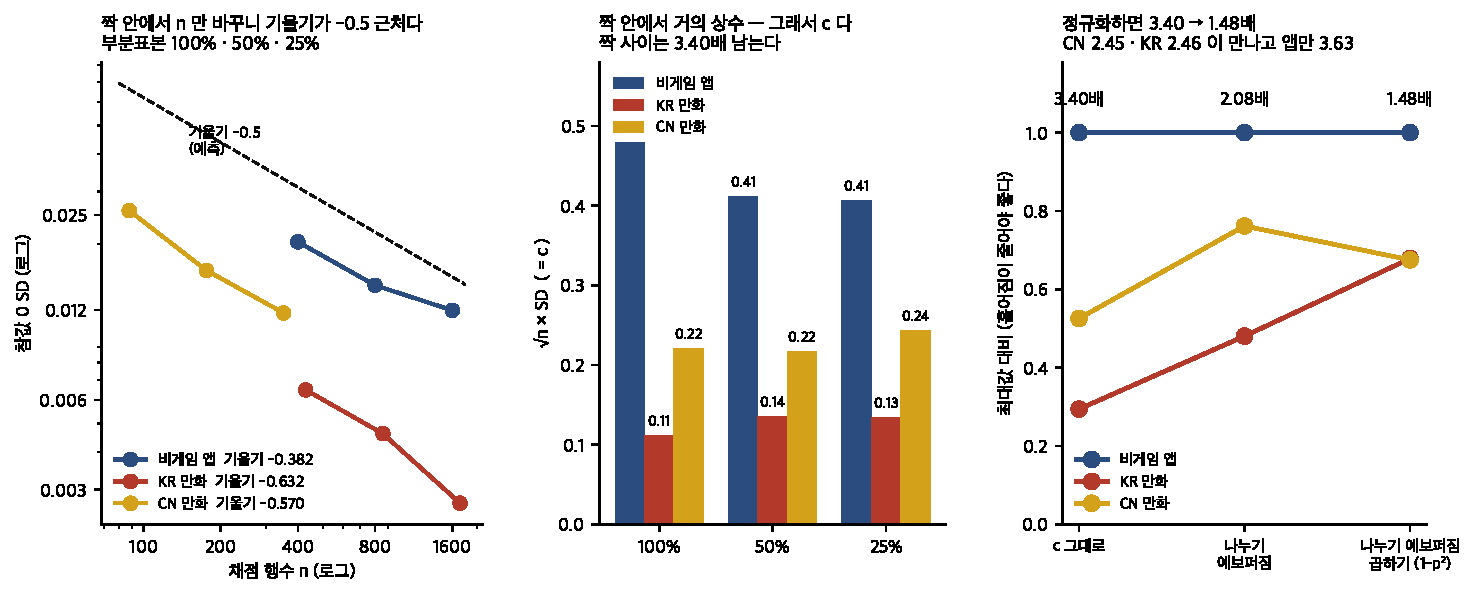
\includegraphics[width=0.99\textwidth]{figs/noiselaw.pdf}
\caption{왼쪽: 로그--로그. \textbf{짝 안 기울기가 $-0.5$ 근처다.} 가운데:
$\sqrt{n}\times$SD --- \textbf{짝 안에서 거의 상수}이고 짝 사이는 $3.40$배 남는다.
오른쪽: 정규화 사다리 --- $3.40 \to 2.08 \to 1.48$배.}
\end{figure}

\section{지수가 확인됐다}

\begin{center}
\begin{tabular}{lrrrr}
\toprule
짝 & 로그--로그 기울기 & \multicolumn{3}{c}{$\sqrt{n}\times$SD ($=c$)} \\
 & (예측 $-0.5$) & $100\%$ & $50\%$ & $25\%$ \\
\midrule
비게임 앱 & $\mathbf{-0.382}$ & $0.479$ & $0.411$ & $0.407$ \\
KR 만화 & $\mathbf{-0.632}$ & $0.112$ & $0.135$ & $0.134$ \\
CN 만화 & $\mathbf{-0.570}$ & $0.220$ & $0.216$ & $0.243$ \\
\midrule
평균 & $-0.53$ & \multicolumn{3}{l}{짝 안에서 거의 상수 --- 그래서 $c$ 다} \\
\bottomrule
\end{tabular}
\end{center}

셋 다 사전등록 범위($-0.35$--$-0.65$) 안이고, \textbf{$\sqrt{n}\times$SD 가 짝 안에서
상수}라는 것이 같은 사실의 다른 표현이다.

\claim{\textbf{참값 $0$ SD $= c(\text{짝})/\sqrt{n}$.} 지수는 표본 크기에서 오는
것이고 짝마다 같다. \textbf{그래서 문턱 $= 2\sqrt{2}\,c/\sqrt{n}$ 로 계산할 수 있고
짝마다 $c$ 를 한 번만 재면 된다.} ($\sqrt{2}$ 는 문턱이 \emph{두 팔의 차}에 걸리기
때문이다.)}
{앱의 기울기가 $-0.382$ 로 $-0.5$ 에서 가장 멀다. 부분표본을 더 잘게($12.5\%$) 넣어
기울기가 계속 $-0.4$ 근처면 앱에서는 다른 항이 섞인 것이고, $c$ 를 상수로 쓸 수
없다.}

\subsection*{노트 715 와 $\sqrt{2}$ 로 이어진다}

노트 715 는 \textbf{위약 쌍의 차} SD 를 쟀고 이 논문은 \textbf{한 팔} SD 를 쟀다.
독립이면 차의 SD $=\sqrt{2}\times$ 한 팔 SD 여야 한다. 실측 비 --- 앱 $0.91$ ·
KR $1.05$ · CN $0.72$. 둘은 $10\%$ 안이고 CN 만 어긋나는데 \textbf{노트 715 의 CN
은 셔플 4 뿐}이었다(여기는 20).

\claim{\textbf{두 측정이 서로를 검증한다.} 설계가 다르고($4$ 셔플의 쌍차 대 $20$
셔플의 팔 SD) 목적이 다른데 $\sqrt{2}$ 관계로 맞는다. 그래서 어느 쪽도 배선 사고가
아니다.}
{셔플을 더 늘렸을 때 CN 의 비가 $0.72$ 에서 $1$ 로 안 오면 그 짝에서 두 팔이 독립이
아니라는 뜻이고, 그러면 $\sqrt{2}$ 를 쓸 수 없다.}

\section{남는 것 --- $c$ 가 3.4배 다르다}

$c$ 는 앱 $0.432$ · CN $0.227$ · KR $0.127$ 로 \textbf{$3.40$배} 범위다. 그리고
\textbf{같은 $n$ 에서도 실재한다} --- $25\%$ 층에서 앱($n=400$) SD $0.0203$ 대
KR($n=429$) SD $0.0065$ 로 \textbf{$3.1$배}다. 행수가 거의 같다.

\begin{center}
\begin{tabular}{lrrr}
\toprule
정규화 & 앱 & CN & KR \\
\midrule
$c$ 그대로 & $0.432$ & $0.227$ & $0.127$ \\
$\div$ 예보 퍼짐 & $2.73$ & $2.08$ & $1.31$ \\
$\div$ 예보 퍼짐 $\times (1-\rho^2)$ & $3.63$ & $\mathbf{2.45}$ & $\mathbf{2.46}$ \\
\midrule
흩어짐 & \multicolumn{3}{l}{$3.40 \to 2.08 \to \mathbf{1.48}$배} \\
\bottomrule
\end{tabular}
\end{center}

\claim{\textbf{예보 퍼짐만으로는 절반만 설명된다($3.40 \to 2.08$).} $(1-\rho^2)$ 를
곱하면 $1.48$ 배까지 줄고 \textbf{CN $2.45$ 와 KR $2.46$ 이 만난다}. 기제로는
그럴듯하다 --- 열 하나를 섞으면 예보가 그 열의 퍼짐만큼 흔들리고, 이미 $\rho$ 가
높으면 순위가 확정돼 있어 스피어만이 덜 움직인다.}
{\textbf{$n=3$ 이고 앱이 $1.48$배 남는다. 그러므로 이 형태를 주장하지 않는다} ---
노트 551 · 560 · 563 이 같은 종류의 순서 관측을 세 번 처방으로 바꿨다가 세 번
틀렸다. 넷째 짝이 생길 때 시험한다.}

\subsection*{그리고 $\rho$ 단조는 틀렸다}

사전등록 예측 ③ 은 \emph{``기준선 $\rho$ 가 높으면 $c$ 가 작다''} 였다. KR($\rho\,
0.683$)이 $c$ 최소인 것은 맞지만 \textbf{CN($0.387$)이 앱($0.497$)보다 $c$ 가
작다} --- 단조가 아니다. $\rho$ 는 $(1-\rho^2)$ 꼴로 \emph{다른 항과 곱해질 때만}
일한다.

\section{그래서 문턱이 계산된다 --- 그런데 채택은 안 된다}

새 문턱 $=2\sqrt{2}\,c/\sqrt{n}$:

\begin{center}
\begin{tabular}{lrrrrl}
\toprule
짝 & $n$ & 기록된 문턱 & \textbf{새 문턱} & 신호 몫 & \\
\midrule
비게임 앱 & $1{,}600$ & $0.024$ & $\mathbf{0.0305}$ & $+0.0839$ & \textbf{$2.75$배 통과} \\
KR 만화 & $1{,}716$ & $0.025$ & $\mathbf{0.0087}$ & $+0.0092$ & $1.06$배 \\
CN 만화 & $352$ & $0.022$ & $\mathbf{0.0342}$ & $+0.0053$ & $0.15$배 미달 \\
\bottomrule
\end{tabular}
\end{center}

KR 문턱이 $0.025 \to 0.0087$ 로 \textbf{$2.9$배 낮아진다} --- 옛 문턱이 그 짝에서
$6.2\sigma$ 였기 때문이다.

\claim{\textbf{그래도 채택은 없다.} 규약 12(집 밖 $\ge 2$)를 채우려면 KR 이 필요한데
\textbf{$1.06$배는 못 믿는다} --- 노트 709 의 CN 이 $1.23$배였고 씨앗을 늘리자
무너졌다(노트 710). $1.06$ 은 그보다 얇다. \textbf{이 논문의 값은 ``채택''이 아니라
``문턱을 계산할 수 있게 된 것''이다.}}
{KR 을 씨앗 12 · 셔플 20 으로 굳혀 신호 몫이 $0.0087$ 위에 남으면 집 밖 $2/3$ 로
규약 12 를 충족한다. 그것이 다음 실험이고, \textbf{개정 자체는 노트 714 의 약속대로
따로 사전등록한다.}}

\end{document}
